%---------------------------------------------------
\chapter{Polyphonic support} 
\label{poly}
%---------------------------------------------------

Directly programing polyphonic instruments in \faust is perfectly possible. It is also needed if very complex signal interaction between the different voices have to be described\footnote{Like sympathetic strings resonance in a physical model of a piano for instance.}.

But since all voices would always be computed, this approach could be too CPU costly for simpler or more limited needs. In this case describing a single voice in a \faust DSP program and externally combining several of them with a special  {\it polyphonic instrument aware} architecture file is a better solution. Moreover, this special architecture file takes care of dynamic voice allocations and control MIDI messages decoding and mapping.

\section{Polyphonic ready DSP code}

By convention \faust architecture files with polyphonic capabilities expect to find control parameters named {\it freq}, {\it gain} and {\it gate}.  The metadata \code{declare nvoices "8";}   kind of line with a desired value of  voices can be added in the source code.

In the case of MIDI control, the {\it freq} parameter (which should be a frequency) will be automatically computed from MIDI note numbers, {\it gain} (which should be a value between 0 and 1) from velocity and {\it gate} from {\it keyon/keyoff} events. Thus, gate can be used as a trigger signal for any envelope generator, etc.

\section{Using the mydsp\_poly class}

The single voice has to be described by a \faust DSP program, the \code{mydsp_poly} class is then used to combine several voices and create a polyphonic ready DSP:

\begin{itemize}

\item  the {\it faust/dsp/poly-dsp.h} file contains the definition of the \code{mydsp_poly} class used to wrap the DSP voice into the polyphonic architecture. This class maintains an array of \code{dsp}  type of objects, manage dynamic voice allocations, control MIDI messages decoding and mapping, mixing of all running voices, and stopping a voice when its output level decreases below a given threshold.

\item as a sub-class of DSP, the \code{mydsp_poly}  class redefines the \code{buildUserInterface} method. By convention all allocated voices are grouped in a global  {\it Polyphonic} tabgroup. The first tab contains a {\it Voices} group, a master like component used to change parameters on all voices at the same time, with a {\it Panic} button to be used to stop running voices\footnote{An internal control grouping mechanism has been defined to automatically dispatch a user interface action done on the master component on all linked voices, except for the  {\it freq}, {\it gain} and {\it gate} controls.}, followed by one tab for each voice. Graphical User Interface components will then reflect the multi-voices structure of the new polyphonic DSP (Figure \ref{fig:poly-ui}). 

 \end{itemize}
 
\begin{figure}[!ht]
\begin{center}
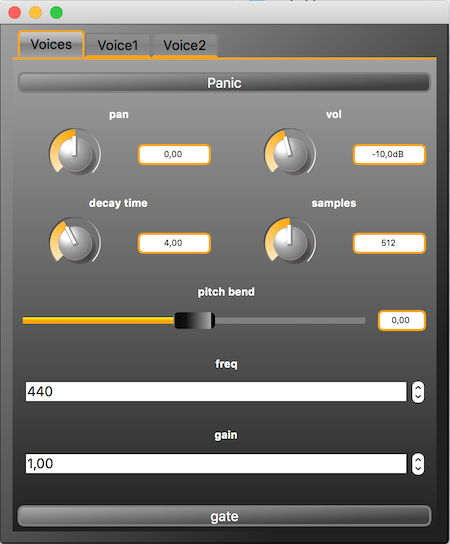
\includegraphics[width=0.6\columnwidth]{images/poly_ui}
\caption{\footnotesize Extended multi-voices GUI interface}
\label{fig:poly-ui}
\end{center}
\end{figure}

The resulting polyphonic DSP object can be used as usual, connected with the needed audio driver, and possibly other UI control objects like OSCUI, httpdUI, etc. Having this new UI hierarchical view allows complete OSC control of each single voice and their control parameters, but also all voices using the master component. 

The following OSC messages reflect the same DSP code either compiled normally,  or in polyphonic mode (only part of the OSC hierarchies are displayed here):

\footnotesize
\begin{lstlisting}

// Mono mode

/0x00/0x00/vol f -10.0
/0x00/0x00/pan f 0.0

// Polyphonic mode

/Polyphonic/Voices/0x00/0x00/pan f 0.0
/Polyphonic/Voices/0x00/0x00/vol f -10.0
...
/Polyphonic/Voice1/0x00/0x00/vol f -10.0
/Polyphonic/Voice1/0x00/0x00/pan f 0.0
...
/Polyphonic/Voice2/0x00/0x00/vol f -10.0
/Polyphonic/Voice2/0x00/0x00/pan f 0.0
...
\end{lstlisting}
\normalsize

The polyphonic instrument allocation takes the DSP to be used for one voice\footnote{The DSP object will be automatically cloned in the mydsp\_poly class to create all needed voices.},  the desired number of voices, the {\it dynamic voice allocation} state\footnote{Voices may be always running, or dynamically started/stopped in case of MIDI control.},  and the {\it group} state which controls if separated voices are displayed or not (Figure \ref{fig:poly-ui}): 

\footnotesize
\begin{lstlisting}
    DSP = new mydsp_poly(dsp, 2, true, true);  
\end{lstlisting}
    
\normalsize
With the following code, note that a polyphonic instrument may be used outside of a MIDI control context, so that all voices will be always running and possibly controlled with OSC messages for instance:

\footnotesize
\begin{lstlisting}
    DSP = new mydsp_poly(dsp, 8, false, true);
\end{lstlisting}

\normalsize
    
\section{Controlling the polyphonic instrument}

The \code{mydsp_poly} class is also ready for MIDI control and can react to {\it keyon/keyoff} and {\it pitchwheel} messages. Other MIDI control parameters can directly be added in the DSP source code. 

\section{Deploying the polyphonic instrument}

Several architecture files and associated scripts have been updated to handle polyphonic instruments:

As an example on OSX, the script \code{faust2caqt foo.dsp} can be used to create a polyphonic CoreAudio/QT application. The desired number of voices is either declared in a \code{nvoices} metadata or changed with the \code{-nvoices num} additional parameter\footnote{-nvoices parameter takes precedence over the  metadata value.}. MIDI control is activated using the \code{-midi} parameter. 

The number of allocated voices can possibly be changed at runtime using the \code{-nvoices} parameter to change the default value (so using \code{./foo -nvoices 16} for instance). 

Several other scripts have been adapted using the same conventions.

\section{Polyphonic instrument with a global output effect}

Polyphonic instruments may be used with an output effect. Putting that effect in the main \faust code is not a good idea since it would be instantiated for each voice which would be very inefficient. This is a typical use case for the  \code{dsp_sequencer} class previously presented with the polyphonic DSP connected in sequence with a unique global effect (Figure \ref{fig:poly-ui-effect}). 

\code{faustcaqt inst.dsp -effect effect.dsp} with inst.dsp and effect.dsp in the same folder,  and the number of outputs of the instrument matching the number of inputs of the effect, has to be used. A \code{dsp_sequencer} object will be created to combine the polyphonic instrument in sequence with the single output effect. 

Polyphonic ready  {\it faust2xx} scripts will then compile the polyphonic instrument and the effect, combine them in sequence, and create a ready to use DSP.  

\begin{figure}[!ht]
\begin{center}
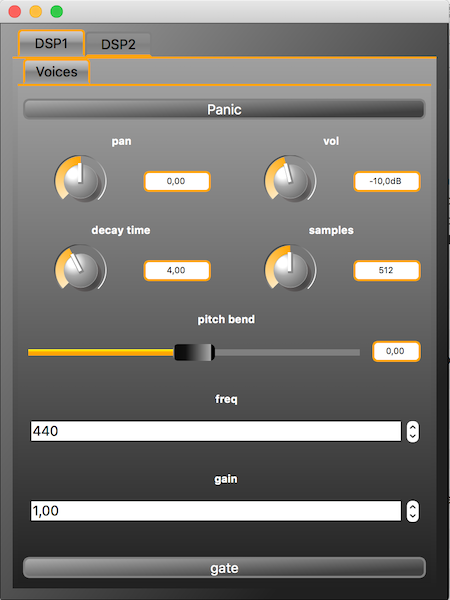
\includegraphics[width=0.48\columnwidth]{images/poly_ui_effect1}
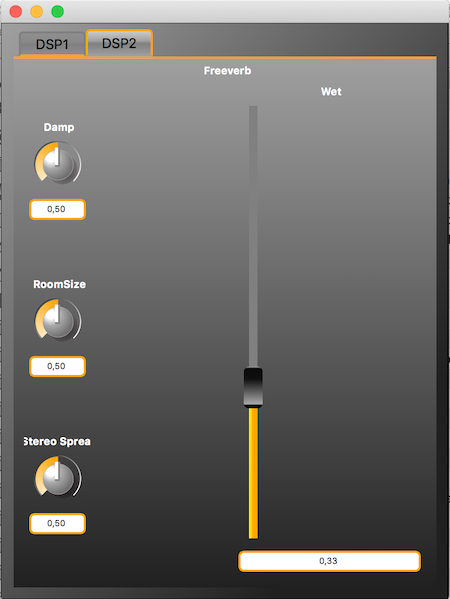
\includegraphics[width=0.48\columnwidth]{images/poly_ui_effect2}
\caption{\footnotesize Polyphonic instrument with output effect GUI interface: left tab window shows the polyphonic instrument with its {\it Voices} group only, right tab window shows the output effect.}
\label{fig:poly-ui-effect}
\end{center}
\end{figure}

\subsection{Integrated global output effect}

Starting with the 2.5.17 version, a new convention has been defined to directly integrate a global output effect inside the DSP source code itself. The effect has simply to be declared in a \code{effect =  effect_code;} line in the source. Here is a more complete source code example:

\begin{lstlisting}
import("stdfaust.lib");
process = pm.clarinet_ui_MIDI <: _,_;
effect = dm.freeverb_demo;
\end{lstlisting}

The architecture script then separates the instrument description itself (the \code{process = ...} definition) from the effect definition (the  \code{effect = ...} definition), possibly adapts the instrument number of outputs to the effect number of inputs, compiles each part separately, and combines them with the \code{dsp_sequencer} object.

A new \code{auto} parameter to be used in {\it faust2xx} script has been defined, as in the \code{faustcaqt inst.dsp -effect auto} line for example.

\subsection{Integrated global output effect and libfaust}

For developers using the libfaust library, an helper file named \code{faust/dsp/poly-dsp-tools.h} is available. It defines an API to automatically create a polyphonic instrument with an output effect, starting from a DSP source file using the  effect \code{effect = ...} convention. The function \code{createPolyDSPFactoryFromString} or  \\ \code{createPolyDSPFactoryFromFile} must be used to create the polyphonic DSP factory. Next, the \code{createPolyDSPInstance} function creates the polyphonic object (a subclass of \code{dsp_poly} type) to be used like a regular \code{dsp} type object. 

After the DSP factory has been compiled, your application or plugin may want to save/restore it in order to save \faust to LLVM IR compilation or even JIT compilation time at next use. To get the internal factory compiled code, several functions are available:

\begin{itemize}
\item \code{writePolyDSPFactoryToIRFile} allows to save the polyphonic factory LLVM IR (in textual format) in a file,
\item \code{writePolyDSPFactoryToBitcodeFile} allows to save the polyphonic factory LLVM IR (in binary format) in a file,
\item \code{writePolyDSPFactoryToMachineFile} allows to save the polyphonic factory executable machine code in a file.
\end{itemize}

To re-create a DSP factory from a previously saved code, several functions are available:

\begin{itemize}
\item \code{readPolyDSPFactoryFromIRFile} allows to create a polyphonic DSP factory from a file containing the LLVM IR (in textual format),
\item \code{readPolyDSPFactoryFromBitcodeFile} allows to create a polyphonic  factory from a file containing the LLVM IR (in binary format),
\item \code{readPolyDSPFactoryFromMachineFile} allows to create a polyphonic DSP factory from a file containing the executable machine code.
\end{itemize}
